\documentclass[12pt,a4paper]{report}

\usepackage[french]{babel}
\usepackage[T1]{fontenc}
\usepackage[utf8]{inputenc}
\usepackage{wrapfig}
\usepackage{graphicx}
\graphicspath{{./Images/}}
\usepackage{float}
\usepackage{amsmath}
\usepackage{amssymb}
\usepackage{xcolor}
\usepackage[]{minted}
\usemintedstyle{emacs}

\definecolor{bgwhite}{HTML}{ffffff}

\usepackage{hyperref}
\hypersetup{
    %bookmarks=true,                                                    % show or hide the bookmarks bar when displaying the document
    unicode=true,                                                       % allows to use characters of non-Latin based languages in Acrobat’s bookmarks
    colorlinks=true,                                                    % surround the links by color frames (false) or colors the text of the links (true). The color of these links can be configured using the following options (default colors are shown)
    linkcolor=black,                                                    % color of internal links (sections, pages, etc.)
    citecolor=yellow,                                                   % color of citation links (bibliography)
    filecolor=orange,                                                   % color of file links
    urlcolor=blue,                                                      % color of URL links (mail, web)
    pdftoolbar=true,                                                    % show or hide Acrobat’s toolbar
    pdfmenubar=true,                                                    % show or hide Acrobat’s menu
    pdffitwindow=false,                                                 % resize document window to fit document size
    pdfstartview={FitH},                                                % fit the width of the page to the window
    pdftitle={Systeme Complexe},                                        % define the title that gets displayed in the "Document Info" window of Acrobat
    pdfauthor={David HONG},                                             % the name of the PDF’s author, it works like the one above
    pdfsubject={Systeme Complexe, Model checking, LTL, CTL, Python, LaTeX},                                                   % subject of the document, it works like the one above
    pdfcreator={David HONG},                                            % creator of the document, it works like the one above
    pdfproducer={David HONG},                                           % producer of the document, it works like the one above
    pdfkeywords={David HONG, Systeme Complexe, Model checking, LTL, CTL, Python, LaTeX},     % list of keywords, separated by commas
    pdfnewwindow=true,                                                  % define if a new PDF window should get opened when a link leads out of the current document
    %pagebackref=true,                                                  % activate back references inside bibliography
    linkbordercolor={1 1 0},                                            % color of frame around internal links 
    citebordercolor={0 1 0},                                            % color of frame around citations
    urlbordercolor={0 0 1}                                              % color of frame around URL links
}

\begin{document}

\begin{titlepage}
    \begin{sffamily}
    \begin{center}
        \begin{flushright}
            \includegraphics[scale=0.25]{Institut-Galilee.png}~\\[7.5cm]
        \end{flushright}
        { \huge \bfseries Rapport système complexe\\[1.0cm] }
        {\large \today \\[1.0cm]}
        \LARGE David HONG
    \end{center}
    \end{sffamily}
\end{titlepage}

\setcounter{tocdepth}{2}
\tableofcontents
\newpage

\chapter*{Introduction}
\addcontentsline{toc}{section}{Introduction}

\paragraph{}On va implémenter les algorithmes de model checking vu en cours des formules CTL. Il existe 6 cas.

\begin{enumerate}
    \item $\phi = p$
    \item $\phi = \neg\psi$
    \item $\phi = \psi1 \land \psi2$
    \item $\phi = EX\psi$
    \item $\phi = E\ \psi1\ U\ \psi2$
    \item $\phi = A\ \psi1\ U\ \psi2$
\end{enumerate}

\paragraph{}Voici tous les fichiers :
\begin{itemize}
    \item Un rapport expliquant les structures de données utilisées, choix d'implémentations, perspectives d'amélioration et application sur quelques exemples.
    \item Un fichier \verb+README.MD+ contenant les instructions.
    \item Un dossier \verb+src+ contenant les codes en python.
    \item Un dossier \verb+images+ contenant des captures d'écran.
    \item Un fichier \verb+in.txt+ contenant la description textuelle d'une structure de Kripke et d'une formule CTL. Et aussi un fichier \verb+in.txt.bak+ pourla structure de Kripke et la formule CTL par défaut.
\end{itemize}

\newpage

\section*{Structure de Kripke}
\addcontentsline{toc}{section}{Structure de Kripke}

\paragraph{}Une structure de Kripke peut être représentée par
\begin{itemize}
    \item Un ensemble d'états.
    \item Un ensemble de transitions.
\end{itemize}

\paragraph{}On a plusieurs méthodes pour les structures de Kripke :
\begin{itemize}
    \item \verb+get_etats+ elle renvoie l'ensemble des états.
    \item \verb+get_transitions+ elle renvoie l'ensemble des transitions.
    \item \verb+add_etat+ elle ajoute un état à la structure de Kripke.
    \item \verb+add_transition+ elle ajoute une transition à la structure de Kripke.
    \item \verb+nb_etats+ elle renvoie le nombre d'états de la structure de Kripke.
    \item \verb+nb_transitions+ elle renvoie le nombre de transitions de la structure de Kripke.
    \item \verb+etat_in+ test si un état est dans la structure de Kripke.
    \item \verb+transition_in+ test si une transition est dans la structure de Kripke.
    \item \verb+print_transition+ affiche la structure de Kripke en affichant les états et les transitions.
\end{itemize}

\paragraph{}Il y a aussi les méthodes pour le model checker.

\paragraph{}Nous allons donc faire deux autres structures une qui représente les états et une autre les transitions.

\section*{Etat}
\addcontentsline{toc}{section}{Etat}

\paragraph{}Un état est un couple qui contient un entier et un ensemble de propositions. On suppose que l'entier est positif ou nul.

\paragraph{Exemple:}\verb+Etat(0, ['req1'])+ est un état où \verb+req1+ est vrai dans cet état.

\paragraph{}On a plusieurs méthodes pour les états :
\begin{itemize}
    \item \verb+get_etat+ elle renvoie l'état.
    \item \verb+get_props+ elle renvoie les propositions qui sont vérifiées.
    \item \verb+print_etat+ elle affiche l'état.
\end{itemize}

\section*{Transition}
\addcontentsline{toc}{section}{Transition}

\paragraph{}Une transition est un couple d'entier source et destination. On suppose que les entiers sont positifs ou nuls.

\paragraph{Exemple:}\verb+Transition(0, 1)+ est une transition qui part de 0 jusqu'à 1.

\paragraph{}On a plusieurs méthodes pour les transitions :

\begin{itemize}
    \item \verb+get_source+ elle renvoie l'état source de la transition.
    \item \verb+get_destination+ elle renvoie l'état destination de la transition.
    \item \verb+print_transition+ elle affiche la transition.
\end{itemize}

\section*{Le model checker}
\addcontentsline{toc}{section}{Le model checker}

\paragraph{}Il faut implémenter les différents cas. Il suffit de suivre les algorithmes vue en cours pour l'implémentation.

\subsection*{Cas 1 : $\phi = p$}
\addcontentsline{toc}{subsection}{Cas 1 : $\phi = p$}

\begin{minted}[
    frame=lines,
    framesep=2mm,
    baselinestretch=1.2,
    bgcolor=bgwhite,
    fontsize=\footnotesize,
    linenos,
    tabsize=2,
    breaklines
]{python}
def check_prop(self, prop):
    """
    Cas 1
    @param prop: la proposition à vérifier.
    @return res: un dict (etat: bool)
    """
    res = {}
    # Pour tous les états
    for e in self.etats:
        # prop est dans la liste des propositions atomiques donc True
        if prop in e.get_props():
            res[e.get_etat()] = True
        # prop n'est pas dans la liste des propositions atomiques donc False
        else:
            res[e.get_etat()] = False
    return res
\end{minted}

\subsection*{Cas 2 : $\phi = \neg \psi$}
\addcontentsline{toc}{subsection}{Cas 2 : $\phi = \neg \psi$}

\begin{minted}[
    frame=lines,
    framesep=2mm,
    baselinestretch=1.2,
    bgcolor=bgwhite,
    fontsize=\footnotesize,
    linenos,
    tabsize=2,
    breaklines
]{python}
def check_not(self, prop):
    """
    Cas 2
    @param prop: la proposition à vérifier ou un dict
    @return res: un dict (etat: bool)
    """
    res = {}
    # prop est une proposition
    if isinstance(prop, str):
        # On transforme prop en un dict (marking(phi))
        prop = self.check_prop(prop)
    # On parcours tous les propositions de prop
    for i, j in prop.items():
        # On a un True donc on aura False
        if j == True:
            res[i] = False
        # On a False donc on aura True
        else:
            res[i] = True
    return res
\end{minted}

\subsection*{Cas 3 : $\phi = \psi_{1} \land \psi_{2}$}
\addcontentsline{toc}{subsection}{Cas 3 : $\phi = \psi_{1} \land \psi_{2}$}

\begin{minted}[
    frame=lines,
    framesep=2mm,
    baselinestretch=1.2,
    bgcolor=bgwhite,
    fontsize=\footnotesize,
    linenos,
    tabsize=2,
    breaklines
]{python}
def check_and(self, prop1, prop2):
    """
    Cas 3
    @param prop1: la proposition à vérifier ou un dict.
    @param prop2: la proposition à vérifier ou un dict.
    @return res: un dict (etat: bool)
    """
    res = {}
    # prop est un string
    if isinstance(prop1, str) and isinstance(prop2, str):
        mark_prop1 = self.check_prop(prop1)
        mark_prop2 = self.check_prop(prop2)
        for i in self.etats:
            res[i.get_etat()] = mark_prop1[i.get_etat()] and mark_prop2[i.get_etat()]
    # prop est un dict
    else:
        for i, j in prop1.items():
            res[i] = prop1[i] and prop2[i]        
    return res
\end{minted}

\subsection*{Cas 4 : $\phi = EX \psi$}
\addcontentsline{toc}{subsection}{Cas 4 : $\phi = EX \psi$}

\begin{minted}[
    frame=lines,
    framesep=2mm,
    baselinestretch=1.2,
    bgcolor=bgwhite,
    fontsize=\footnotesize,
    linenos,
    tabsize=2,
    breaklines
]{python}
def check_next(self, prop):
    """
    Cas 4
    @param prop: la proposition à vérifier ou un dict.
    @return res: un dict (etat: bool)
    """
    res = {}
    # On initialise tous à False
    for i in self.etats:
        res[i.get_etat()] = False
    # prop est une proposition
    if isinstance(prop, str):
        # On transforme prop en un dict (marking(phi))
        prop = self.check_prop(prop)
    # On parcours les transitions
    for t in self.transitions:
        # On a trouvé une transition qui à l'état destination à vrai
        if prop[t.get_destination()] == True:
            res[t.get_source()] = True
    return res
\end{minted}

\subsection*{Cas 5 : $\phi = E \psi_{1} U \psi_{2}$}
\addcontentsline{toc}{subsection}{Cas 5 : $\phi = E \psi_{1} U \psi_{2}$}

\begin{minted}[
    frame=lines,
    framesep=2mm,
    baselinestretch=1.2,
    bgcolor=bgwhite,
    fontsize=\footnotesize,
    linenos,
    tabsize=2,
    breaklines
]{python}
def check_euntil(self, prop1, prop2):
    """
    Cas 5
    @param prop1: la proposition à vérifier ou un dict.
    @param prop2: la proposition à vérifier ou un dict.
    @return res: un dict (etat: bool)
    """
    res = {}
    L = []
    seenbefore = {}
    # Initialise tout à False et seenbefore à False
    for q in self.etats:
        res[q.get_etat()] = False
        seenbefore[q.get_etat()] = False
    # prop1 est une proposition
    if isinstance(prop1, str):
        # On transforme prop1 en un dict (marking(phi1))
        prop1 = self.check_prop(prop1)
    # prop2 est une proposition
    if isinstance(prop2, str):
        # On transforme prop2 en un dict (marking(phi2))
        prop2 = self.check_prop(prop2)
    # On parcours tous les états
    for q in self.etats:
        # L'état q est vrai dans prop2 (phi2)
        if prop2[q.get_etat()] == True:
            # On ajout l'état q dans la liste L
            L.append(q.get_etat())
    # On parcours la liste l tant qu'elle n'est pas vide
    while len(L) != 0:
        # On prend un état q dans la liste L
        for q in L:
            # On met à True
            res[q] = True
            # On parcours tous les transitions
            for t in self.transitions:
                # On a trouve une transition entrant vers q
                if t.get_destination() == q:
                    if seenbefore[t.get_source()] == False:
                        seenbefore[t.get_source()] = True
                        if prop1[t.get_source()] == True:
                            L.append(t.get_source())
        # On enlève q de la liste L
        L.pop(-1)
    return res
\end{minted}

\subsection*{Cas 6 : $\phi = A \psi_{1} U \psi_{2}$}
\addcontentsline{toc}{subsection}{Cas 6 : $\phi = A \psi_{1} U \psi_{2}$}

\begin{minted}[
    frame=lines,
    framesep=2mm,
    baselinestretch=1.2,
    bgcolor=bgwhite,
    fontsize=\footnotesize,
    linenos,
    tabsize=2,
    breaklines
]{python}
def check_auntil(self, prop1, prop2):
    """
    Cas 6
    @param prop1: la proposition à vérifier ou un dict.
    @param prop2: la proposition à vérifier ou un dict.
    @return res: un dict (etat: bool)
    """
    res = {}
    L = []
    degree = {}
    # Initialise tout à False et les degrés de tous les états
    for q in self.etats:
        res[q.get_etat()] = False
        degree[q.get_etat()] = self.get_degree(q.get_etat())
    # prop1 est une proposition
    if isinstance(prop1, str):
        # On transforme prop1 en un dict (marking(phi1))
        prop1 = self.check_prop(prop1)
    # prop2 est une proposition
    if isinstance(prop2, str):
        # On transforme prop2 en un dict (marking(phi2))
        prop2 = self.check_prop(prop2)
    # On parcours tous les états
    for q in self.etats:
        # L'état q est vrai dans prop2 (phi2)
        if prop2[q.get_etat()] == True:
            # On ajout l'état q dans la liste L
            L.append(q.get_etat())
    # On parcours la liste l tant qu'elle n'est pas vide
    while len(L) != 0:
        # On prend un état q dans la liste L
        for q in L:
            # On met à True
            res[q] = True
            # On parcours tous les transitions
            for t in self.transitions:
                # On a trouve une transition entrant vers q
                if t.get_destination() == q:
                    # On décrémente son dégré
                    degree[t.get_source()] -= 1
                    if degree[t.get_source()] == 0 and prop1[t.get_source()] == True and res[t.get_source()] == False:
                        L.append(t.get_source())
            # On enlève q de la liste L
            L.pop(0)
    return res
    
def get_degree(self, n):
    """
    Calcul le degrée d'un état
    @param n: un entier correspondant à l'état
    @return int: le degré sortant
    """
    res = 0
    if isinstance(n, int):
        for i in self.transitions:
            if i.get_source() == n:
                res += 1
    else:
        raise TypeError("L'argument n'est pas un entier !")
    return res
\end{minted}

\section*{Le fichier main}
\addcontentsline{toc}{section}{Le fichier main}

\paragraph{}C'est là que nous allons tester la structure de Kripke entré dans le fichier \verb+in.txt+
\paragraph{}Dans un terminal, tapez \verb+python3 main+

\paragraph{}Dans le main, il y plusieurs fonction :

\begin{itemize}
    \item \verb+KS_bool+ qui construit un dictionnaire d'entier, booléen.
    \item \verb+charger_kripke+ qui va lire le fichier texte et initialiser la structure de Kripke.
    \item \verb+charger_formule+ qui va lire la dernière ligne du fichier et initialiser la formule CTL à tester.
    \item \verb+get_etats_verifie+ qui va renvoyer un ensemble d'états qui sont vrais.
\end{itemize}

\section*{Utilisation}
\addcontentsline{toc}{section}{Utilisation}

\subsection*{Créer sa propre stucture de Kripke}
\addcontentsline{toc}{subsection}{Créer sa propre stucture de Kripke}

\paragraph{}Pour créer sa propre structure de Kripke, il faut modifier le fichier \verb+in.txt+, ce fichier doit contenir les etats et les transitions.

\paragraph{}Il faut ajouter les états en premiers car lorsque l'on ajoute une transition, elle requiert les états source et destination, or si notre structure de Kripke ne possède pas d'état, on aura une exception.

\paragraph{}Sur chaque ligne, on va commencer par mettre une lettre qui indique si la ligne est un état ou une transition (\verb+e+ pour un état, \verb+t+ pour une transition, \verb+f+ pour la formule).

\paragraph{}La dernière ligne du fichier sera la formule CTL.

\paragraph{}Pour les états, on va mettre un entier qui sera le numéro de l'état, puis une suite de propositions atomiques qui sont vérifiés dans cet état.

\begin{minted}[
    frame=lines,
    framesep=2mm,
    baselinestretch=1.2,
    bgcolor=bgwhite,
    fontsize=\footnotesize,
    linenos,
    tabsize=2,
    breaklines
]{text}
e 1 p q
e 2 p
e 3 q
\end{minted}

\paragraph{}Pour les transitions, on va mettre deux entiers, le premier pour l'état source, et la deuxième pour l'état destination.

\begin{minted}[
    frame=lines,
    framesep=2mm,
    baselinestretch=1.2,
    bgcolor=bgwhite,
    fontsize=\footnotesize,
    linenos,
    tabsize=2,
    breaklines
]{text}
t 1 2
t 2 3
t 3 3
\end{minted}

\paragraph{}Pour la formule, on mettra la séquence d'exécution de notre model checker. On utilise les mots-clés qui sont :

\begin{itemize}
    \item \verb+True+
    \item \verb+False+
    \item \verb+not+ pour le non logique
    \item \verb+and+ pour le et logique
    \item \verb+next+ pour le next
    \item \verb+euntil+ pour le exist until
    \item \verb+auntil+ pour le always until
\end{itemize}

\begin{minted}[
    frame=lines,
    framesep=2mm,
    baselinestretch=1.2,
    bgcolor=bgwhite,
    fontsize=\footnotesize,
    linenos,
    tabsize=2,
    breaklines
]{text}
f and p q
\end{minted}

\paragraph{}Cette formule correspond à $p \land q$

\paragraph{}Lancer le \verb+main.py+ et notre structure de Kripke est crée et notre model checker va vérifier la formule CTL dans la structure de Kripke crée.

\paragraph{}Voici quelques exemples :

\begin{figure}[H]
  \centering
      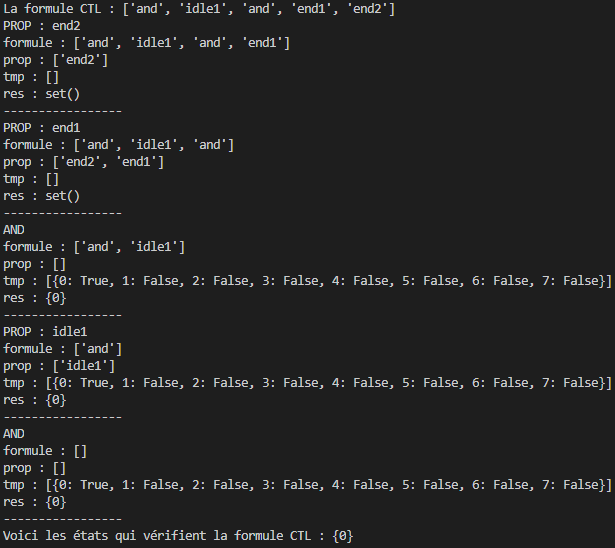
\includegraphics[scale=0.75]{Images/resultat_main_1.PNG}
  \caption{Formule $idle_{1}\land (end_{1} \land end_{2})$ (f and idle1 and end1 end2)}
\end{figure}

\begin{figure}[H]
  \centering
      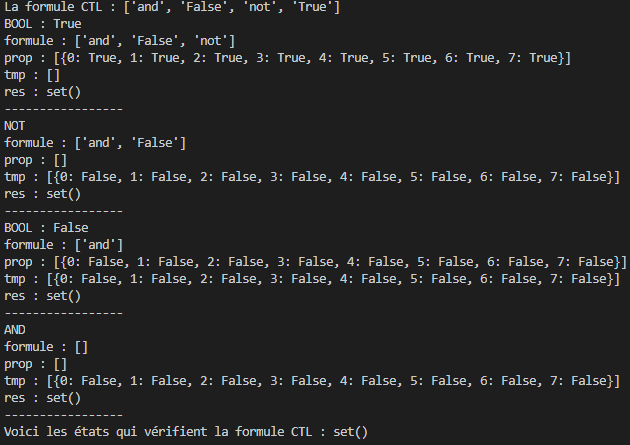
\includegraphics[scale=0.75]{Images/resultat_main_2.PNG}
  \caption{Formule $False\land (\neg True)$ (f and False not True)}
\end{figure}

\section*{Exemples}
\addcontentsline{toc}{section}{Exemples}

\paragraph{}Nous allons tester notre model checker sur quelques exemples vue en cours. Dans le fichier \verb+test.py+ il y a la structure de Kripke de l'exclusion mutuelle (la structure de Kripke dans cet exemple à été crée directement dans le fichier) voici son contenu :

\begin{figure}[H]
  \centering
      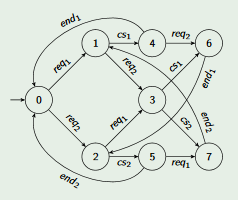
\includegraphics[scale=1]{Images/exclusion_mutuelle.PNG}
  \caption{Exemple de l'exclusion mutuelle}
\end{figure}

\begin{minted}[
    frame=lines,
    framesep=2mm,
    baselinestretch=1.2,
    bgcolor=bgwhite,
    fontsize=\footnotesize,
    linenos,
    tabsize=2,
    breaklines
]{python}
# On créer une structure de Kripke de l'exclusion mutuelle
K = Kripke()
# On ajoute les états
K.add_etat(Etat(0, ["end1", "end2", "idle1", "idle2"]))
K.add_etat(Etat(1, ["req1", "end2", "idle2"]))
K.add_etat(Etat(2, ["req2", "end1", "idle1"]))
K.add_etat(Etat(3, ["req1", "req2"]))
K.add_etat(Etat(4, ["cs1", "idle2"]))
K.add_etat(Etat(5, ["cs2", "idle1"]))
K.add_etat(Etat(6, ["req2", "cs1"]))
K.add_etat(Etat(7, ["req1", "cs2"]))
# On ajoute les transitions
K.add_transition(Transition(0, 1))
K.add_transition(Transition(0, 2))
K.add_transition(Transition(1, 3))
K.add_transition(Transition(1, 4))
K.add_transition(Transition(2, 3))
K.add_transition(Transition(2, 5))
K.add_transition(Transition(3, 6))
K.add_transition(Transition(3, 7))
K.add_transition(Transition(4, 0))
K.add_transition(Transition(4, 6))
K.add_transition(Transition(5, 0))
K.add_transition(Transition(5, 7))
K.add_transition(Transition(6, 2))
K.add_transition(Transition(7, 1))

# Cas 1
checker_prop = K.check_prop("req1")
# Cas 2
checker_not = K.check_not("req1")
# Cas 3
checker_and = K.check_and("req1", "req2")
# Cas 4
checker_next = K.check_next("req1")
# Cas 5
checker_euntil = K.check_euntil("req1", "cs1")
# Cas 6
checker_auntil = K.check_auntil("req1", "cs1")
# Exemple sur une formule CTL
checker_formule1 = K.check_not(K.check_euntil(KS_true(K.nb_etats()), K.check_not(K.check_euntil(KS_true(K.nb_etats()), K.check_and(K.check_prop("idle1"), K.check_prop("idle2"))))))
checker_formule2 = K.check_not(K.check_and(K.check_prop("end1"), K.check_prop("end2")))
checker_formule3 = K.check_and(K.check_and(K.check_prop("req1"), K.check_prop("req2")), K.check_prop("req2"))

print("Cas 1 : {}".format(get_etats_verifie(checker_prop)))
print("Cas 2 : {}".format(get_etats_verifie(checker_not)))
print("Cas 3 : {}".format(get_etats_verifie(checker_and)))
print("Cas 4 : {}".format(get_etats_verifie(checker_next)))
print("Cas 5 : {}".format(get_etats_verifie(checker_euntil)))
print("Cas 6 : {}".format(get_etats_verifie(checker_auntil)))
print("Exemple sur la formule 1 CTL : {}".format(get_etats_verifie(checker_formule1)))
print("Exemple sur la formule 2 CTL : {}".format(get_etats_verifie(checker_formule2)))
print("Exemple sur la formule 3 CTL : {}".format(get_etats_verifie(checker_formule3)))
\end{minted}

\paragraph{}Nous allons tester quelques formules sur tous les cas.
\begin{enumerate}
    \item $\phi = req_{1}$
    \item $\phi = \neg req_{1}$
    \item $\phi = req_{1} \land req_{2}$
    \item $\phi = EX\ req_{1}$
    \item $\phi = E\ req_{1}\ U\ cs_{1}$
    \item $\phi = A\ req_{1}\ U\ cs_{1}$
    \item $\phi = \neg(E\ true\ U\ \neg(E(true\ U\ (idle_{1}\land idle_{2}))))$
    \item $\phi = \neg(end_{1}\land end_{2})$
    \item $\phi = (req_{1}\land req_{2})\land req_{1}$
\end{enumerate}

\paragraph{}On peux tester ces formules dans le fichier \verb+in.txt+ 
\begin{enumerate}
    \item \verb+f req1+
    \item \verb+f not req1+
    \item \verb+f and req1 req2+
    \item \verb+f next req1+
    \item \verb+f euntil req1 cs1+
    \item \verb+f auntil req1 cs1+
    \item \verb+f not euntil True not euntil True and idle1 idle2+
    \item \verb+f not and end1 end2+
    \item \verb+f and and req1 req2 req1+
\end{enumerate}

\paragraph{}Pour tester ces cas, il suffit tapez dans un terminal \verb+python3 test.py+

\paragraph{}Voici les résultats :

\begin{figure}[H]
  \centering
      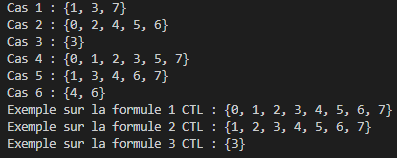
\includegraphics[scale=1]{Images/resultats_test.PNG}
  \caption{Résultats des différents cas}
\end{figure}

\paragraph{}Les 6 cas on été vu en cours, voici les résultats :

\begin{figure}[H]
  \centering
      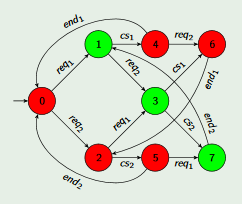
\includegraphics[scale=1]{Images/cas1.PNG}
  \caption{Cas 1}
\end{figure}

\begin{figure}[H]
  \centering
      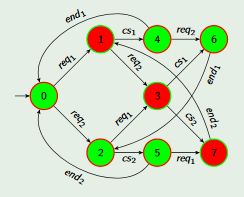
\includegraphics[scale=1]{Images/cas2.PNG}
  \caption{Cas 2}
\end{figure}

\begin{figure}[H]
  \centering
      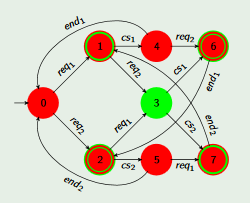
\includegraphics[scale=1]{Images/cas3.PNG}
  \caption{Cas 3}
\end{figure}

\begin{figure}[H]
  \centering
      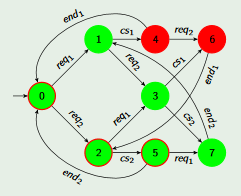
\includegraphics[scale=1]{Images/cas4.PNG}
  \caption{Cas 4}
\end{figure}

\begin{figure}[H]
  \centering
      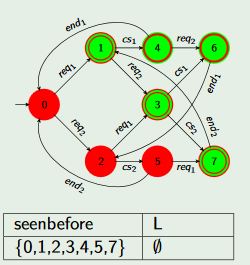
\includegraphics[scale=1]{Images/cas5.PNG}
  \caption{Cas 5}
\end{figure}

\begin{figure}[H]
  \centering
      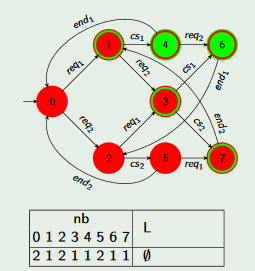
\includegraphics[scale=1]{Images/cas6.PNG}
  \caption{Cas 6}
\end{figure}

\section*{Perspectives d'amélioration}
\addcontentsline{toc}{section}{Perspectives d'amélioration}

\begin{itemize}
    \item Vérifier que le fichier \verb+in.txt+ est correcte.
    \item Vérifier que la formule CTL entré est syntaxiquement correcte (\verb+f not+ n'est pas valide)
    \item 
    \item La conversion automatique des formules CTL (transformation des $\Rightarrow$, $\lor$, etc.)
    \item Faire un model checker sur les formules LTL
    \item Essayer de faire ce projet avec des réseaux de pétri
    \item Améliorer du code
    \item Afficher la structure de Kripke avec un graphe
\end{itemize}

\end{document}